\chapter{剪切自锁问题}
本章讨论另一个自锁问题,中厚板的剪切自锁问题。同样介绍目前常用的罚函数法和拉格朗日乘子法两种解决方法。上文提出的最优约束比同样适用于剪切自锁问题。

\section{中厚板问题}    
考虑如图\ref{mindlin_picture}所示中厚板,其中中板厚为$h$,$\Omega$为板中面。在Mindlin假设下,中厚板考虑横向剪切变形,相应的混合控制方程由下式给出:
\begin{equation}\label{strong_mindlin}
    \begin{cases}
        M_{\alpha\beta,\beta} - Q_\alpha = 0 & \textrm{in}\; \Omega \\
        Q_{\alpha,\alpha} + \bar q = 0 & \textrm{in}\; \Omega \\    Q_\alpha n_\alpha = \bar Q & \textrm{on}\; \Gamma_Q \\
        M_{\alpha\beta} n_\beta = \bar M_\alpha & \textrm{on}\; \Gamma_M \\
        \varphi_\alpha = \bar \varphi_\alpha & \textrm{on}\; \Gamma_\varphi \\
        w = \bar w & \textrm{on}\; \Gamma_w \\
    \end{cases}
\end{equation}
\begin{figure}[H]
    \centering 
        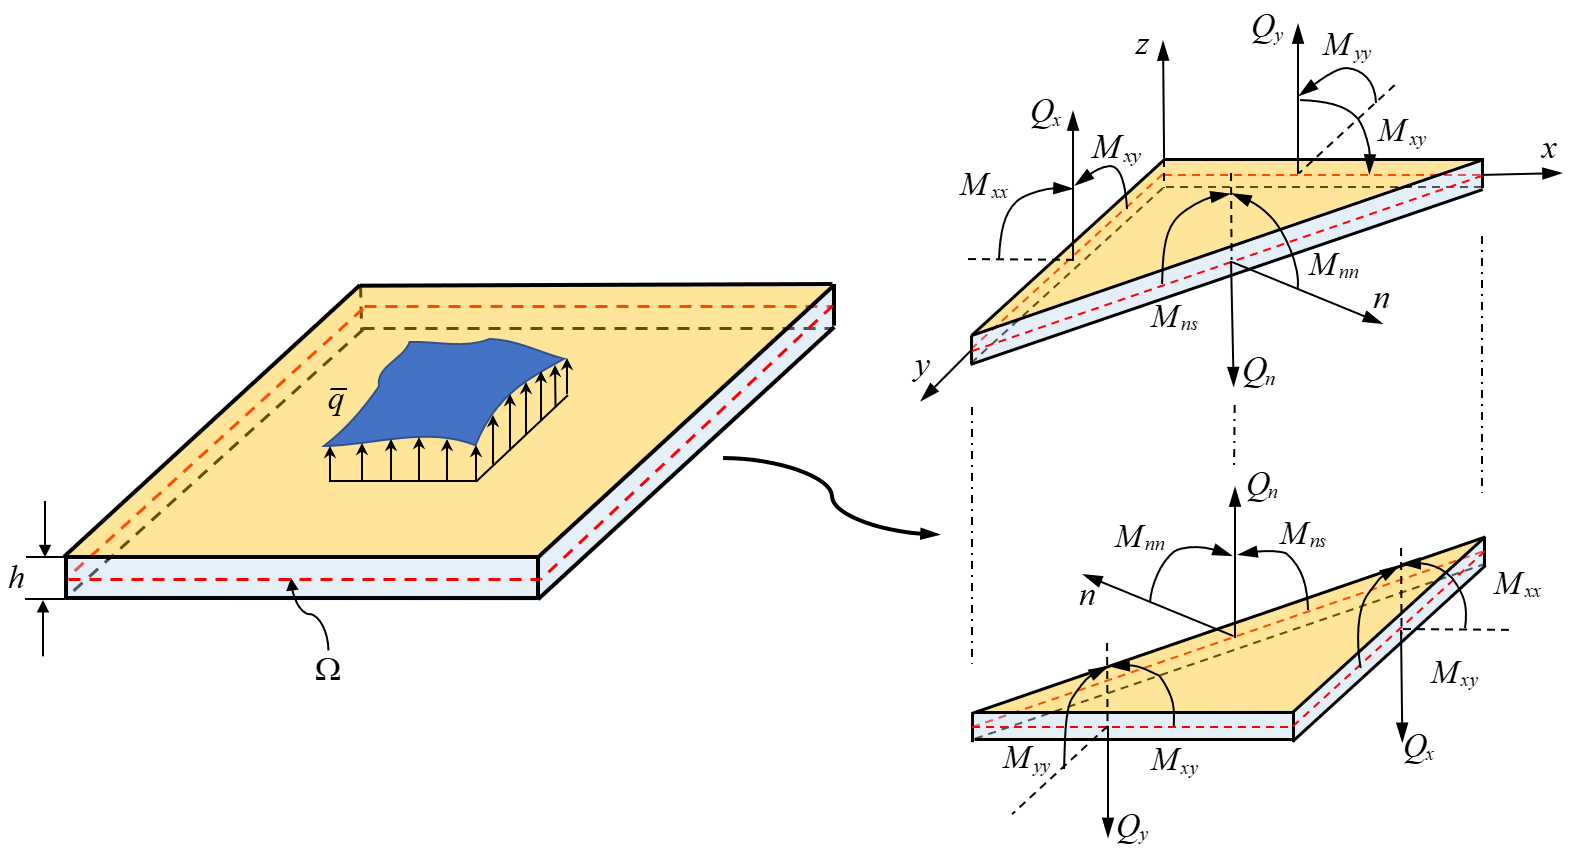
\includegraphics[scale=0.5]{figures/shearlocking/Mindlinplate.png}
        \caption{中厚板运动学及边界条件}\label{mindlin_picture}
\end{figure}
式中,$M_{\alpha \beta}$ 可表示弯矩张量$ \boldsymbol{M}$ 的弯曲或扭转部分的分量,$Q_\alpha$为剪力张量$\boldsymbol{Q}$的分量,$\bar{q}$ 为垂直于板中面的分布荷载;
$\Gamma_w$和$\Gamma_\varphi$为本质边界条件,$\bar{w}$和$\bar{\varphi}_\alpha$分别为本质边界条件上给定的挠度和转角;
$\Gamma_Q$ 和$\Gamma_M$ 为自然边界条件,$\bar Q$和$\bar{M}_{\alpha}$ 为自然边界上的等效剪力和法向弯矩;
$n_\alpha$为边界上外法线方向$\pmb{n}$的分量。

在平面应力假设下,对于各同向性线弹性材料,其本构关系表示为:
\begin{equation}\label{mindlin_M}
    M_{\alpha \beta}=-\frac{h^3}{12}D_{\alpha \beta \gamma\eta}\kappa_{\gamma\eta}=\frac{h^3}{12}D_{\alpha \beta \gamma\eta}\varphi_{\gamma,\eta}
\end{equation}
\begin{equation}\label{mindlin_Q}
    Q_{\alpha}=k\frac{Eh}{2(1+\nu)}\gamma_\beta=kGh(-\varphi_\beta+w_{,\beta})
\end{equation}
其中,$k$为剪切修正系数,$\kappa_{\alpha\beta}$为曲率张量$\pmb\kappa$的分量,$\gamma_\alpha$为剪切应变矢量$\pmb\gamma$的分量,表达式为:
\begin{equation} \label{kappa}
    \kappa_{\alpha\beta}=-\varphi_{\alpha,\beta},\quad\gamma_\alpha=-\varphi_\alpha+w_{,\alpha}
\end{equation}
式中$D_{\alpha \beta \gamma\eta}$为在平面应力假设下四阶弹性张量的分量,表达式为:
\begin{equation} 
    D_{\alpha \beta \gamma\eta}=\frac{E}{1-\nu^2}(\nu\delta_{\alpha\beta}\delta_{\gamma\eta}+\frac{1}{2}(1-\nu)(\delta_{\alpha\gamma}\delta_{\beta\eta}+\delta_{\alpha\eta}\delta_{\beta\gamma}))
\end{equation}

根据最小势能原理,强形式\eqref{strong_mindlin}所对应的势能泛函表达式为: 
\begin{equation}\label{potential_energy}
    \begin{split} 
        \Pi(w,\boldsymbol{\varphi})&=\frac{1}{2}\int_{\Omega}\kappa_{\alpha\beta}M_{\alpha\beta}d\Omega+\frac{1}{2}\int_{\Omega}\gamma_{\alpha}Q_{\alpha}d\Omega\\
        &+\int_{\Gamma_{M}}\varphi_{\alpha}{\bar{M}_{\alpha}}d\Gamma-\int_{\Gamma_{Q}}{w}\bar {Q}d\Gamma-\int_{\Omega} w\bar{q}d\Omega
    \end{split}
\end{equation}
对式\eqref{potential_energy}进行变分可得弱形式:
挠度,转角$(w,\varphi_{\alpha})\in V$,使
\begin{equation}\label{weak_penalty_mindlin}
    \begin{split} 
        &\int_{\Omega}\delta\kappa_{\alpha\beta}M_{\alpha\beta}d\Omega+\int_{\Omega}\delta\gamma_{\alpha}Q_{\alpha}d\Omega=\\
        &-\int_{\Gamma_{M}}\delta\varphi_{\alpha}{\bar{M}_{\alpha}}d\Gamma+\int_{\Gamma_{Q}}{\delta{w}}\bar {Q}d\Gamma+\int_{\Omega} \delta{w}\bar{q}d\Omega,\quad \forall(\delta w,\delta\varphi_{\alpha}) \in V
    \end{split}
\end{equation}

对于考虑横向剪切变形的中厚板,根据中厚板的本构关系\eqref{mindlin_M},\eqref{mindlin_Q},当其厚度减小$h\rightarrow 0$,弯矩$M_{\alpha \beta}$减小的速度远大于剪力$Q_{\alpha}$,使得$Q_{\alpha}\gg M_{\alpha \beta}$。在式\eqref{weak_penalty_mindlin}中$Q_{\alpha}\gg M_{\alpha \beta}$,剪切应变$\boldsymbol{\gamma}$被约束,导致板的剪切位移为$0$。

在传统有限元法中,如图\ref{mindlin_fem}所示整个求解域$\Omega$由一组具有节点$\{\boldsymbol x_I\}_{I=1}^{n_u}$的构造网格离散,其中$n_u$是节点的数量。
挠度$w$及其变分$\delta w $,转角$\varphi_\alpha$及其变分$\delta \varphi_\alpha $可通过$x_I$处的节点系数和形函数进行近似:
\begin{equation}\label{w_h}
    w^h(\boldsymbol x) = \sum_{I=1}^{n_u} N_I(\boldsymbol x) w_I, \quad \delta w^h(\boldsymbol x) = \sum_{I=1}^{n_u} N_I(\boldsymbol x) \delta w_I
\end{equation}
\begin{equation}\label{varphi_h}
    \varphi^h_{\alpha}(\boldsymbol x) = \sum_{I=1}^{n_u} N_I(\boldsymbol x) \varphi_{\alpha I}, \quad \delta \varphi^h(\boldsymbol x) = \sum_{I=1}^{n_u} N_I(\boldsymbol x) \delta \varphi_{\alpha I}
\end{equation}
其中,$N_I$为节点$x_I$处的形函数,$w_I$和$\varphi_{\alpha I}$节点系数张量。
\begin{figure}[H]
    \centering 
        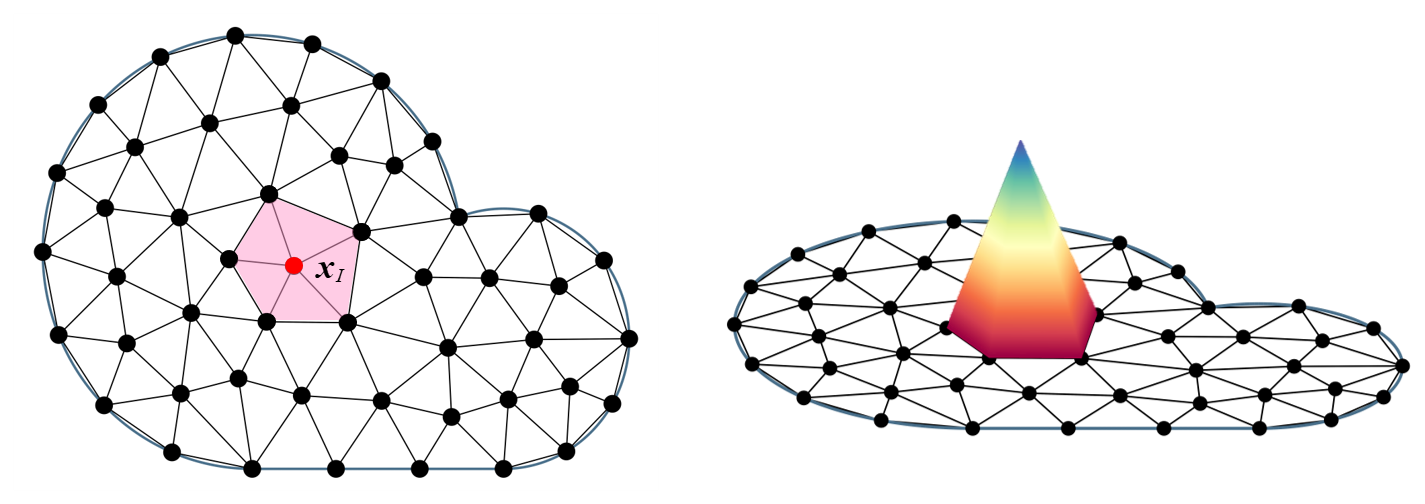
\includegraphics[scale=1.5]{figures/fem.png}
        \caption{有限元离散示意图}\label{mindlin_fem}
\end{figure}

结合式\eqref{kappa},\eqref{w_h}和\eqref{varphi_h},相应的近似曲率$\boldsymbol\kappa$和近似剪切应变$\boldsymbol\gamma$可表示为:
\begin{equation}
    \boldsymbol\kappa^h = 
    \begin{Bmatrix}
        \kappa^h_{11} \\ \kappa^h_{22} \\ 2\kappa^h_{12} 
    \end{Bmatrix} = -\sum_{I=1}^{n_u}
    \begin{bmatrix}
        0 & N_{I,1} & 0 \\ 0 & 0 & N_{I,2} \\ 0 & N_{I,2} & N_{I,1}
    \end{bmatrix}
    \begin{Bmatrix}
        w_I \\ \varphi_{1I} \\ \varphi_{2I}
    \end{Bmatrix} = - \sum_{I=1}^{n_u} \boldsymbol B^b_I \boldsymbol d_I
\end{equation}
\begin{equation}
    \boldsymbol\gamma^h = 
    \begin{Bmatrix}
        \gamma^h_1 \\ \gamma^h_2
    \end{Bmatrix} = \sum_{I=1}^{n_u}
    \begin{bmatrix}
        N_{I,1} & N_I & 0 \\
        N_{I,2} & 0 & N_I
    \end{bmatrix}
    \begin{Bmatrix}
        w_I \\ \varphi_{1I} \\ \varphi_{2I}
    \end{Bmatrix} = \sum_{I=1}^{n_u} \boldsymbol B^s_I \boldsymbol d_I
\end{equation}
\begin{equation}\label{kappa_h}
    \delta\boldsymbol\kappa^h = - \sum_{I=1}^{n_u} \boldsymbol B^b_I \delta\boldsymbol d_I ,\quad \delta\boldsymbol\gamma^h = \sum_{I=1}^{n_u} \boldsymbol B^s_I \delta\boldsymbol d_I
\end{equation}

将式\eqref{kappa_h}代入到弱形式\eqref{weak_penalty_mindlin}可得下列里兹--伽辽金问题:
近似挠度和近似转角$(w^h,\boldsymbol{\varphi}^h_{\alpha})\in V_h$满足
\begin{equation}\label{ritz_penalty_mindlin}
    \begin{split} 
        &\int_{\Omega}\delta\kappa^h_{\alpha\beta}M_{\alpha\beta}d\Omega+\int_{\Omega}\delta\gamma^h_{\alpha}Q_{\alpha}d\Omega=\\
        &-\int_{\Gamma_{M}}\delta\varphi^h_{\alpha}{\bar{M}_{\alpha}}d\Gamma+\int_{\Gamma_{Q}}{\delta{w^h}}\bar {Q}d\Gamma+\int_{\Omega} \delta{w^h}\bar{q}d\Omega,\quad \forall(\delta w^h,\delta\varphi^h_{\alpha}) \in V_h
    \end{split}
\end{equation}
根据$\boldsymbol\kappa^h$和$\boldsymbol\gamma^h$的任意性,上述方程可简化为如下离散控制方程:
\begin{equation}
    (\boldsymbol K^b + \boldsymbol K^s) \boldsymbol d = \boldsymbol f
\end{equation}
其中,$\boldsymbol K^b$为弯曲刚度矩阵,$\boldsymbol K^s$为剪切刚度矩阵,$\pmb{f}$为力矢量,其分量具有以下形式:
\begin{equation}\label{stiffness_bending}
    \boldsymbol K^b_{IJ} = \frac{h^3}{12} \int_\Omega \boldsymbol B^{bT}_I \boldsymbol D \boldsymbol B^b_J d\Omega\\
\end{equation}
\begin{equation}\label{stiffness_shear}
    \boldsymbol K^s_{IJ} = h \int_\Omega \boldsymbol B^{sT}_I kG \boldsymbol B^s_J d\Omega
\end{equation}
\begin{equation}
    \boldsymbol f_I = \int_{\Gamma_Q} N_I \bar{\boldsymbol Q} d\Gamma - \int_{\Gamma_M} N_I \bar{\boldsymbol M} d\Gamma + \int_\Omega N_I \bar{\boldsymbol q} d\Omega
\end{equation}
式中,$\boldsymbol{D}$为平面应力弹性矩阵,等效剪力$\bar{\boldsymbol Q}$,法向弯矩$\bar{\boldsymbol M}$,分布荷载$\bar{\boldsymbol q}$的分量分别为:
\begin{equation}
    \bar{\boldsymbol Q} =  
    \begin{Bmatrix}
        \bar Q \\ 0 \\ 0
    \end{Bmatrix},
        \bar{\boldsymbol M} =
    \begin{Bmatrix}
        0 \\ \bar M_1 \\ \bar M_2
    \end{Bmatrix},
        \bar{\boldsymbol q} =
    \begin{Bmatrix}
        \bar q \\ 0 \\ 0
    \end{Bmatrix}
\end{equation}

\section{免自锁方案}
\subsection{罚函数法与缩减积分方案}
同样,对于中厚板当厚度减小$h\rightarrow 0$,式\eqref{stiffness_shear}中剪切刚度矩阵$\boldsymbol{K^s}$中的模态远大于式\eqref{stiffness_bending}中弯曲刚度矩阵$\boldsymbol{K^b}$中的模态。
此时,剪切刚度矩阵$\boldsymbol{K^s}$可视为一种强制使用的罚函数法使得剪切部分受到约束。使用传统有限元法进行数值分析时位移解会远小于实际情况,就是所谓的剪切自锁现象。